At the other extreme, commitment is made at a block level: Unified EB retains every position in the denoising window until the whole block satisfies its stopping rule.
Here we examine the order in which DiffusionGemma accepts tokens under the Unified EB sampler.
DiffusionGemma accepts tokens in an order strongly biased toward autoregressive, left-to-right generation.
This autoregressive bias results in many denoising slots within a canvas being "wasted" on tokens that have already converged.
As a result, a form of rolling sampler where the window moves incrementally through the sequence rather than block by block becomes increasingly appealing as a way to extend the Pareto frontier.

\begin{figure}[tbp]
\centering
\begin{tikzpicture}[x=0.205cm, y=0.205cm]

\definecolor{cwinfill}{HTML}{9FE1CB}
\definecolor{cwinedge}{HTML}{0F6E56}
\definecolor{camber}{HTML}{E8A13C}
\definecolor{camberedge}{HTML}{A96A0B}
\definecolor{cwaste}{HTML}{C0553C}
\definecolor{cwasteedge}{HTML}{7A2E1C}
\definecolor{cnoise}{HTML}{D3D1C7}
\definecolor{cnoiseedge}{HTML}{888780}
\definecolor{cclean}{HTML}{FFFFFF}
\definecolor{ccleanedge}{HTML}{B4B4A9}
\definecolor{cframe}{HTML}{2B5E94}

\newcommand{\gridcell}[3]{%
  \ifcase#3\relax
  \or \fill[cwinfill!65, draw=cwinedge,   line width=0.3pt, rounded corners=0.5pt] (#1, -#2) rectangle ++(0.88, -0.88);
  \or \fill[camber!45,   draw=camberedge, line width=0.3pt, rounded corners=0.5pt] (#1, -#2) rectangle ++(0.88, -0.88);
  \or \fill[cwaste,      draw=cwasteedge, line width=0.3pt, rounded corners=0.5pt] (#1, -#2) rectangle ++(0.88, -0.88);
  \or \fill[cclean,      draw=ccleanedge, line width=0.3pt, rounded corners=0.5pt] (#1, -#2) rectangle ++(0.88, -0.88);
  \or \fill[cnoise,      draw=cnoiseedge, line width=0.3pt, rounded corners=0.5pt] (#1, -#2) rectangle ++(0.88, -0.88);
  \fi}

\newcommand{\gridrow}[4]{%
  \foreach \c in {0,...,23} {%
    \pgfmathtruncatemacro{\sty}{\c<#3 ? 4 : (\c<#4 ? 1 : 5)}%
    \pgfmathsetmacro{\xpos}{\c + #1}%
    \gridcell{\xpos}{#2}{\sty}%
  }}

\newcommand{\gridmarks}[4]{%
  \foreach \c in {#4} {%
    \pgfmathsetmacro{\xpos}{\c + #1}%
    \gridcell{\xpos}{#2}{#3}%
  }}

\newcommand{\keydenoise}{\begin{tikzpicture}[baseline=-0.5ex, x=0.30cm, y=0.30cm]
  \fill[cwinfill!65, draw=cwinedge, line width=0.3pt, rounded corners=0.5pt] (0,-0.5) rectangle ++(0.88,1);
\end{tikzpicture}}
\newcommand{\keyaccept}{
\begin{tikzpicture}[baseline=-0.5ex, x=0.30cm, y=0.30cm]
  \fill[camber!45, draw=camberedge, line width=0.3pt, rounded corners=0.5pt] (0,-0.5) rectangle ++(0.88,1);
\end{tikzpicture}}
\newcommand{\keywaste}{
\begin{tikzpicture}[baseline=-0.5ex, x=0.30cm, y=0.30cm]
  \fill[cwaste, draw=cwasteedge, line width=0.3pt, rounded corners=0.5pt] (0,-0.5) rectangle ++(0.88,1);
\end{tikzpicture}}
\newcommand{\keycache}{
\begin{tikzpicture}[baseline=-0.5ex, x=0.30cm, y=0.30cm]
  \fill[cclean, draw=ccleanedge, line width=0.3pt, rounded corners=0.5pt] (0,-0.5) rectangle ++(0.88,1);
\end{tikzpicture}}
\newcommand{\keyunadmitted}{
\begin{tikzpicture}[baseline=-0.5ex, x=0.30cm, y=0.30cm]
  \fill[cnoise, draw=cnoiseedge, line width=0.3pt, rounded corners=0.5pt] (0,-0.5) rectangle ++(0.88,1);
\end{tikzpicture}}

\node[anchor=west, font=\footnotesize\bfseries] at (0, 1.5) {(a) Block sampler, $b=8$: 19 passes};

\gridrow{0}{0}{0}{8}
\gridrow{0}{1}{0}{8}
\gridrow{0}{2}{0}{8}                     \gridmarks{0}{2}{2}{0,3}
\gridrow{0}{3}{0}{8} \gridmarks{0}{3}{3}{0,3}          \gridmarks{0}{3}{2}{1,2}
\gridrow{0}{4}{0}{8} \gridmarks{0}{4}{3}{0,1,2,3}      \gridmarks{0}{4}{2}{4,6}
\gridrow{0}{5}{0}{8} \gridmarks{0}{5}{3}{0,1,2,3,4,6}  \gridmarks{0}{5}{2}{5,7}
\gridrow{0}{6}{8}{16}
\gridrow{0}{7}{8}{16}
\gridrow{0}{8}{8}{16}                        \gridmarks{0}{8}{2}{8,11}
\gridrow{0}{9}{8}{16}  \gridmarks{0}{9}{3}{8,11}             \gridmarks{0}{9}{2}{9}
\gridrow{0}{10}{8}{16} \gridmarks{0}{10}{3}{8,9,11}          \gridmarks{0}{10}{2}{10,13}
\gridrow{0}{11}{8}{16} \gridmarks{0}{11}{3}{8,9,10,11,13}    \gridmarks{0}{11}{2}{12,14}
\gridrow{0}{12}{8}{16} \gridmarks{0}{12}{3}{8,9,10,11,12,13,14} \gridmarks{0}{12}{2}{15}
\gridrow{0}{13}{16}{24}
\gridrow{0}{14}{16}{24}
\gridrow{0}{15}{16}{24}                          \gridmarks{0}{15}{2}{16,19}
\gridrow{0}{16}{16}{24} \gridmarks{0}{16}{3}{16,19}              \gridmarks{0}{16}{2}{17,18}
\gridrow{0}{17}{16}{24} \gridmarks{0}{17}{3}{16,17,18,19}        \gridmarks{0}{17}{2}{20,22}
\gridrow{0}{18}{16}{24} \gridmarks{0}{18}{3}{16,17,18,19,20,22}  \gridmarks{0}{18}{2}{21,23}

\foreach \x in {7.94, 15.94} {
  \draw[cframe, dashed, line width=0.4pt] (\x, 0.3) -- (\x, -19.2);
}
\node[anchor=east, font=\scriptsize] at (-0.5, -0.44) {$t=1$};
\node[anchor=east, font=\scriptsize] at (-0.5, -18.44) {$t=19$};

\node[anchor=west, font=\footnotesize\bfseries] at (29.5, 1.5) {(b) Rolling sampler, $w=8$: 13 passes};

\gridrow{29.5}{0}{0}{8}
\gridrow{29.5}{1}{0}{8}
\gridrow{29.5}{2}{0}{8}                          \gridmarks{29.5}{2}{2}{0,3}
\gridrow{29.5}{3}{1}{9}   \gridmarks{29.5}{3}{3}{3}          \gridmarks{29.5}{3}{2}{1,2}
\gridrow{29.5}{4}{4}{12}                         \gridmarks{29.5}{4}{2}{4,6}
\gridrow{29.5}{5}{5}{13}  \gridmarks{29.5}{5}{3}{6}          \gridmarks{29.5}{5}{2}{5,7,8}
\gridrow{29.5}{6}{9}{17}                         \gridmarks{29.5}{6}{2}{9,12}
\gridrow{29.5}{7}{10}{18} \gridmarks{29.5}{7}{3}{12}         \gridmarks{29.5}{7}{2}{10,11}
\gridrow{29.5}{8}{13}{21}                        \gridmarks{29.5}{8}{2}{13,14,17}
\gridrow{29.5}{9}{15}{23} \gridmarks{29.5}{9}{3}{17}         \gridmarks{29.5}{9}{2}{16,18}
\gridrow{29.5}{10}{15}{23} \gridmarks{29.5}{10}{3}{16,17,18} \gridmarks{29.5}{10}{2}{15,19}
\gridrow{29.5}{11}{20}{24}                       \gridmarks{29.5}{11}{2}{20,22}
\gridrow{29.5}{12}{21}{24} \gridmarks{29.5}{12}{3}{22}       \gridmarks{29.5}{12}{2}{21,23}

\node[anchor=east, font=\scriptsize] at (29.0, -0.44) {$t=1$};
\node[anchor=east, font=\scriptsize] at (29.0, -12.44) {$t=13$};

\node[anchor=north, font=\scriptsize, inner sep=0pt] at (26.7, -20.4) {%
  \begin{tabular}{@{}l@{~}l@{\hspace{1.8em}}l@{~}l@{\hspace{1.8em}}l@{~}l@{}}
    \keydenoise & denoising slot   & \keyaccept     & accepted on this pass &
    \keywaste   & wasted: re-denoised while waiting \\[2.5pt]
    \keycache   & in the KV cache  & \keyunadmitted & not yet admitted      &
                &                                    \\
  \end{tabular}};

\end{tikzpicture}
\caption{\textbf{Where the denoising slots go.} Both samplers denoise a
width-$8$ window per pass in the same order, and the colours are those of
Figure~\ref{fig:algorithm-concept}: teal = still denoising, amber = accepted
on this pass, white = already encoded and in the KV cache, gray = not yet
admitted.  Brick marks a slot spent re-denoising a position that was already
accepted but is still waiting for its prefix, that is, wasted work.
\textbf{(a)} The block sampler appends only once the block is fully resolved,
so converged positions idle and each block re-pays warm-up.  \textbf{(b)} The
rolling sampler appends the accepted prefix immediately and admits fresh
positions in its place, wasting far fewer slots.}
\label{fig:block-vs-rolling}
\end{figure}


\paragraph{Defining Redundant Computations}
Here we define what constitutes a redundant computation.
Our goal is to measure the computations that could conceivably be omitted without drastically impacting the model's behavior.
Thus we define wasted denoising slots as positions that have already converged and are part of a contiguous prefix that could be appended to the KV cache.
We illustrate this definition in Figure \ref{fig:block-vs-rolling}, against the ideal sampler that commits them to the KV cache and avoids redundant denoising steps.

\begin{figure}[tbp]
    \centering
    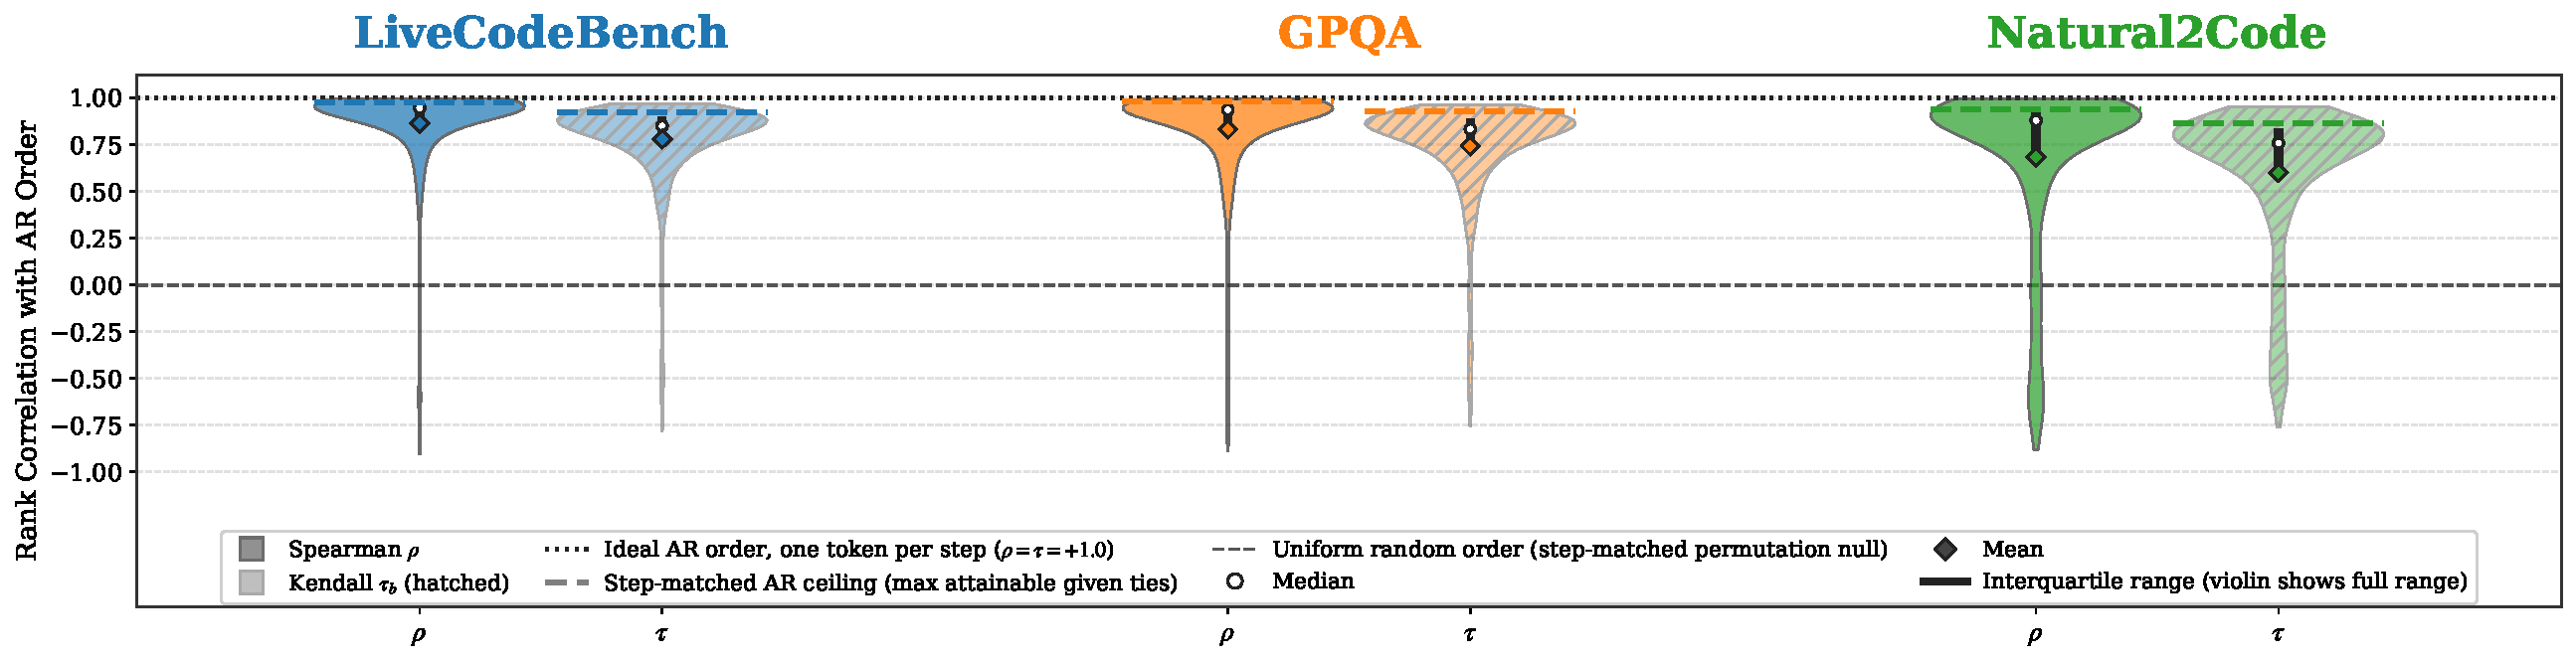
\includegraphics[width=\linewidth]{images/fig_ar_order_correlation_eb0.1_renoise.pdf}

    \vspace{8pt}

    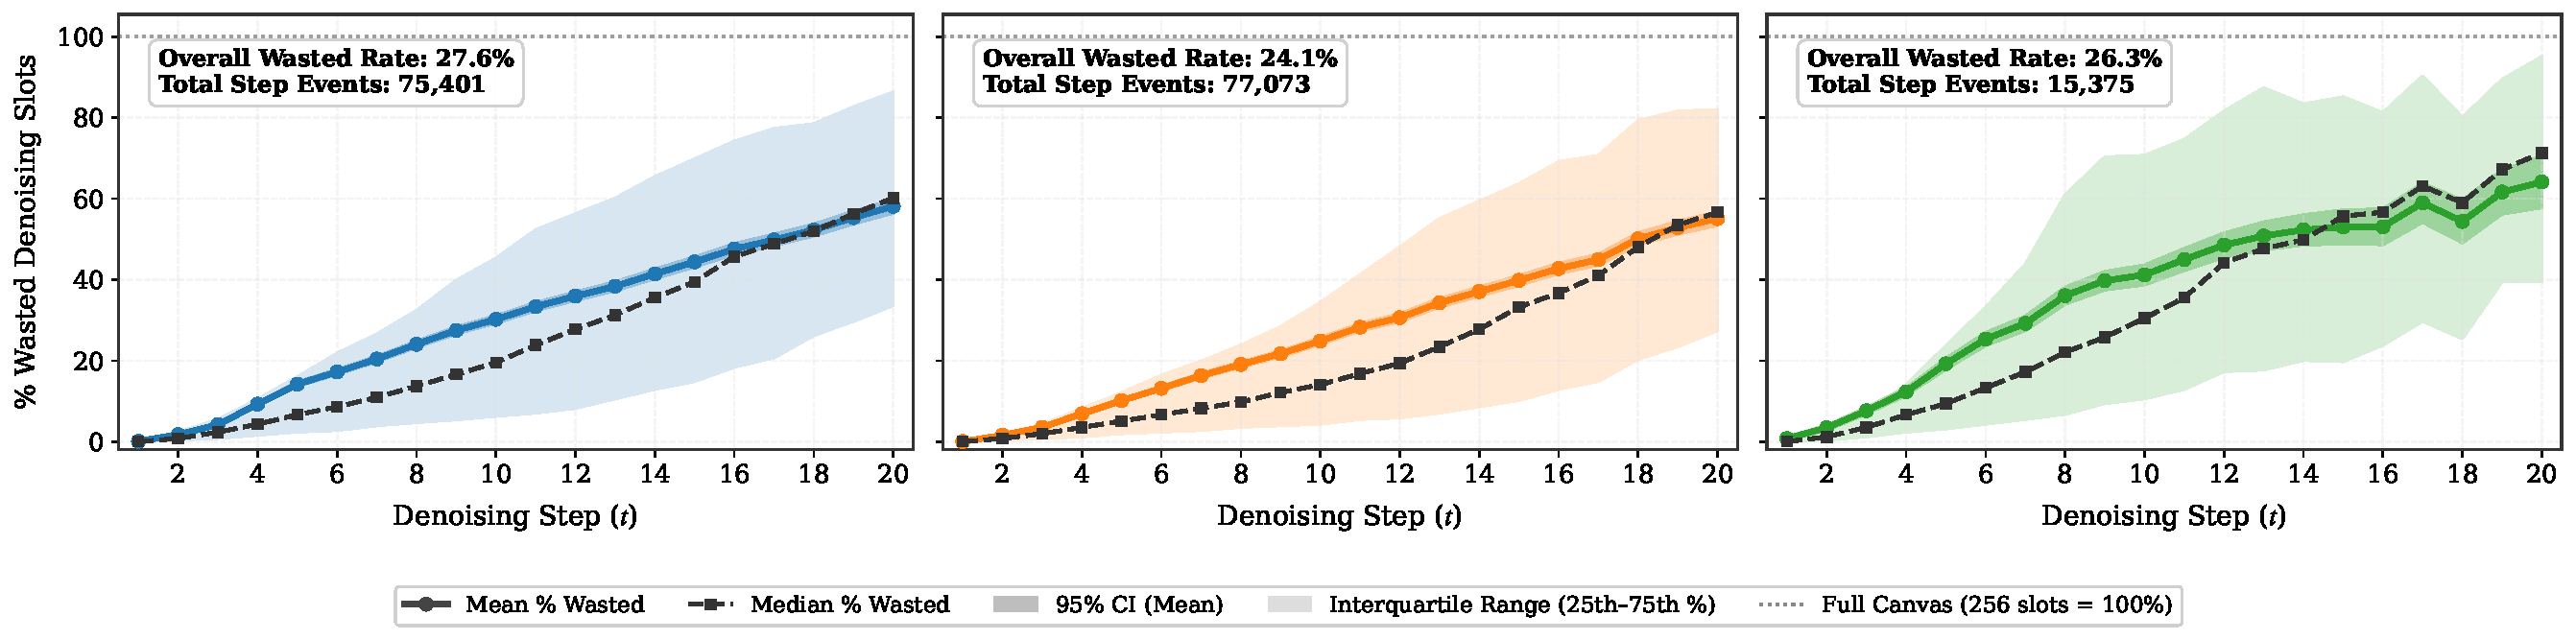
\includegraphics[width=\linewidth]{images/wasted_canvas_slots_lcb_gpqa_n2c.pdf}

    \vspace{8pt}

    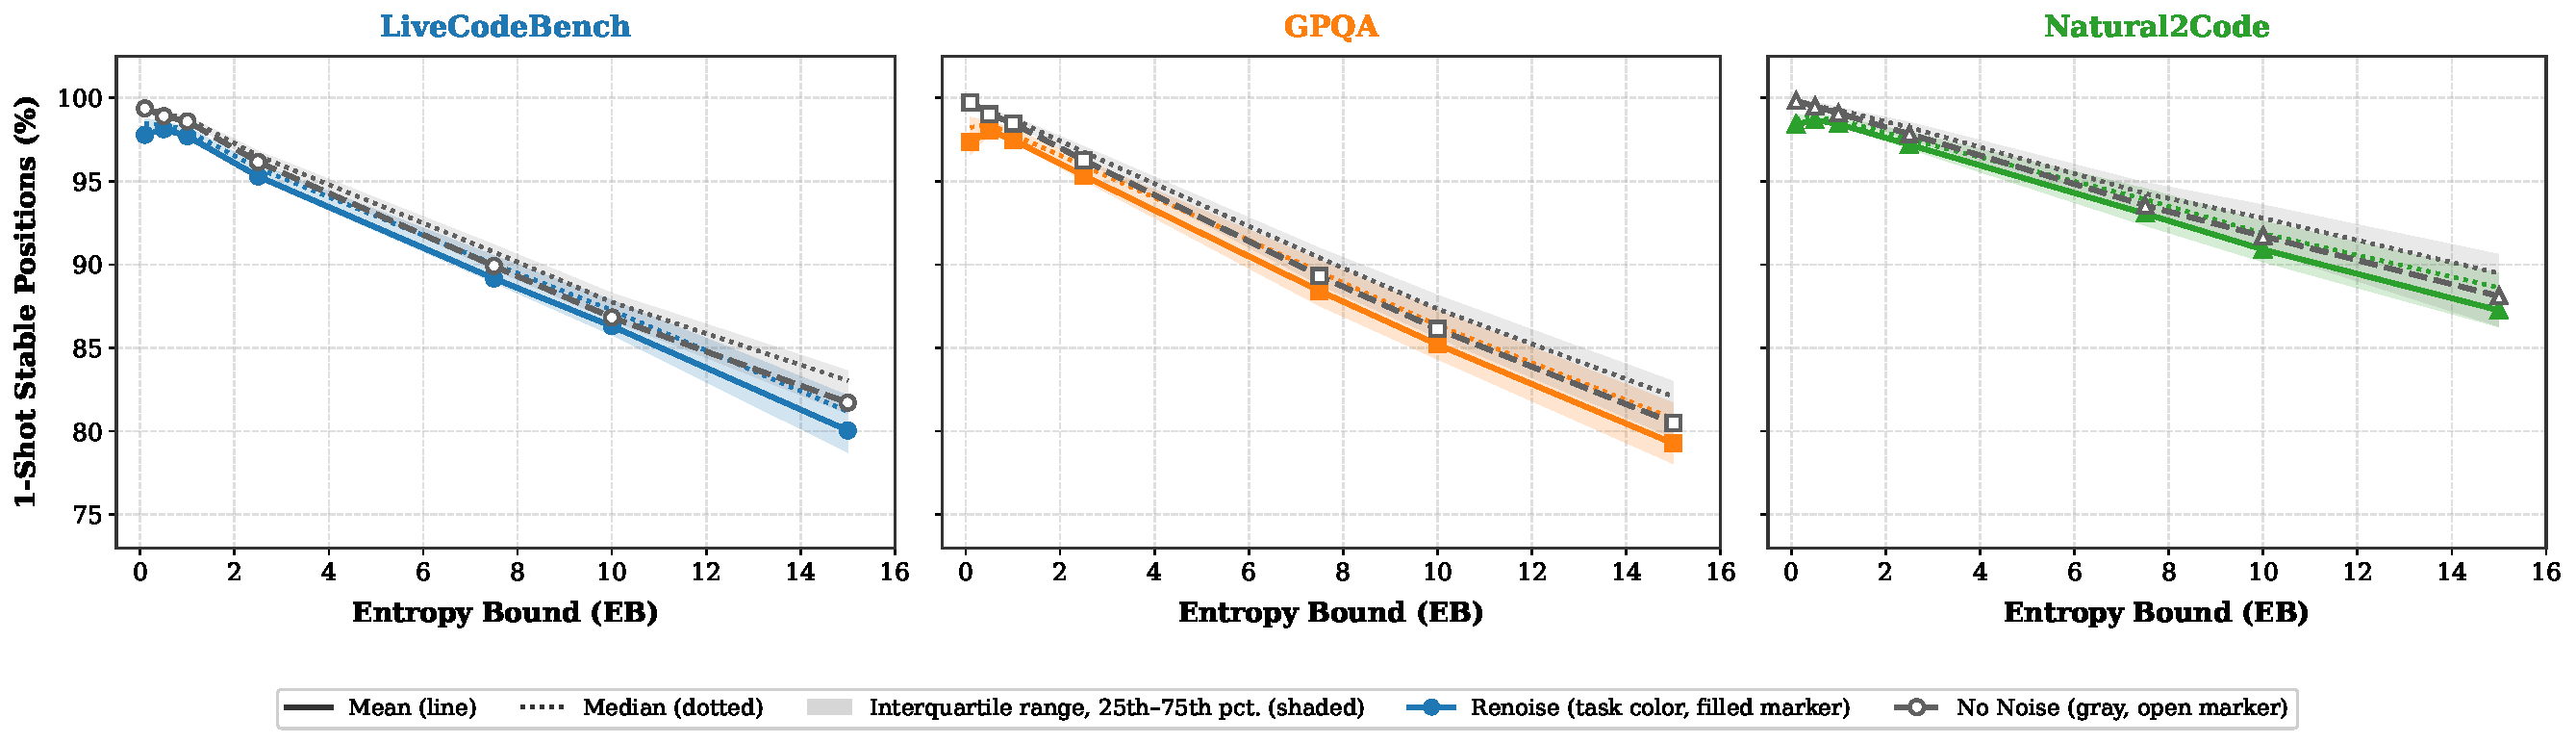
\includegraphics[width=\linewidth,trim=0 0 0 23.5pt,clip]{images/fig_1shot_stability_1x2_row.pdf}
    \caption{Columns in the top and middle rows show LiveCodeBench, GPQA Diamond, and Natural2Code. \textbf{Top row:} Spearman $\rho$ and Kendall $\tau$ between the acceptance order of the DiffusionGemma EB sampler and the AR generation order; across all tasks the sampler is strongly biased towards left-to-right order. \textbf{Middle row:} Percentage of wasted denoising slots averaged across canvases for LCB v6, GPQA Diamond and Natural2Code. For a given sampling step, a slot is wasted if it belongs to a contiguous prefix that has already converged to its final token. By denoising step 20, the mean fraction of wasted canvas slots exceeds 50\% on all three tasks. \textbf{Bottom row:} Accepted tokens are revised more often at higher entropy bounds (in both argmax and sampled-token stability), independent of renoising.}
    \label{fig:wasted}
\end{figure}


\paragraph{Experimental Setup}
We run the Unified EB sampler on LCB v6, GPQA Diamond and Natural2Code. We track the trajectories of each denoising block, and consider a position as converged when it realizes the value that ends up being committed to the KV cache.

\paragraph{Results}
In Figure~\ref{fig:wasted} (top row), we observe that the first-acceptance order is strongly correlated with left-to-right order (Appendix~\ref{app:order-stats}). At the default entropy bound, accepted positions rarely change, so this ordering serves as a proxy for convergence order. This is consistent with the behavior of wasted denoising slots in Figure~\ref{fig:wasted} (middle row), where we observe that the percentage of wasted slots generally increases during the denoising trajectory.

\citet{asaria2026neither} previously observed this autoregressive bias in the DiffusionGemma sampler.
This has been observed as a general pattern for confidence-based samplers across larger diffusion language models \citep{kim2026interface, gong2026diffucoder, lu2026adablock, yao2026decoding}.
\citet{kim2026interface} demonstrates that confidence based samplers tend to generate samples that are very similar to those produced by left-to-right autoregressive order.
Other works demonstrate that the ordering itself is highly left to right and provide various explanations for why \citep{gong2026diffucoder, lu2026adablock, yao2026decoding}.

Convergence in this measurement is identified retrospectively; during sampling, we use EB acceptance as the operational criterion for deciding which positions are ready to commit.
Where per-position commitment loses the chance for later revision, block-level commitment tolerates redundant computation on converged prefixes. Section~\ref{sec:method} introduces RES to strike a balance: wait for a contiguous accepted prefix, without waiting for the entire denoising window.
